\documentclass[11pt,a4paper,openany]{book}
\usepackage[margin=24mm]{geometry}
\usepackage{fontspec}
\IfFontExistsTF{Noto Serif}{\setmainfont{Noto Serif}}{\setmainfont{DejaVu Serif}}
\usepackage{amsmath,amssymb}
\usepackage{tikz}
\usepackage{enumitem}
\usepackage{microtype}
\usepackage[hidelinks]{hyperref}
\setlength{\parindent}{0pt}
\setlength{\parskip}{5pt}
\setlist[enumerate]{leftmargin=*,itemsep=9pt}

\renewcommand{\contentsname}{Mục lục}
\begin{document}
\title{V-TALENT 2045\\ PHY202-A --- Động lực học Newton, ma sát và liên kết\\\large Level 2 · Cơ học nâng cao · Lớp 10–12}
\author{Dr. Dang Minh Tuan -- TS. Đặng Minh Tuấn}
\date{2026 · v1.0}
\maketitle
\tableofcontents
\chapter*{Mục tiêu năng lực}\addcontentsline{toc}{chapter}{Mục tiêu năng lực}
Thiết lập phương trình từ sơ đồ lực; xác định miền ma sát nghỉ, giải động lực học có liên kết, suy điều kiện lăn và kiểm tra giới hạn. Chuẩn bị bài VPhO/TST nhiều chế độ.

Tập chuyên đề đầu tiên, bản thảo 1.0. Bài tập tự biên soạn; chỉ mục đề ngoài dùng để đọc thêm, không sao chép. Cần thẩm định độc lập trước khi dùng đánh giá chính thức.
\chapter{Định luật Newton và các chế độ ma sát}
\section{Lý thuyết và suy luận}
Chọn hệ, hệ quy chiếu quán tính và trục. Định luật II Newton $\sum\vec F_{\rm ext}=d\vec p/dt$ rút gọn thành $m\vec a$ với chất điểm khối lượng không đổi. Nội lực triệt tiêu trong phương trình động lượng toàn hệ nhưng có thể quyết định chuyển động tương đối và nội năng. Trong hệ tịnh tiến phi quán tính gia tốc $\vec A$, đưa vào lực quán tính $-m\vec A$; không trộn gia tốc từ các hệ khác nhau trong một phương trình. Sơ đồ lực chỉ biểu diễn lực tác dụng lên vật đã chọn.

Ma sát Coulomb là mô hình: $|f_s|\le\mu_s N$ khi hai mặt không trượt, và $|f_k|=\mu_k N$ khi trượt, ngược chiều trượt tương đối. Ma sát nghỉ là phản lực liên kết, không mặc nhiên bằng $\mu_sN$. Xác định $N$ từ động lực học vuông góc; không nhất thiết bằng $mg$. Giả sử không trượt, giải lực ma sát cần thiết rồi so sánh độ lớn với $\mu_sN$. Nếu không khả thi, xác định chiều trượt và giải lại với ma sát trượt. Tại $N=0$ phải xem xét lại điều kiện tiếp xúc.

Với hai vật $m$ trên $M$ đặt trên sàn nhẵn, lực ngang $F$ kéo vật dưới, không có gia tốc thẳng đứng, giả thiết không trượt cho $a=F/(M+m)$ và lực ma sát lên vật trên $f=ma$. Do đó $F\le\mu_s(M+m)g$. Vượt ngưỡng (vật dưới trượt về trước so với vật trên), vật trên có $a_m=\mu_k g$, vật dưới $a_M=(F-\mu_k mg)/M$. Kiểm tra $a_M>a_m$ để xác nhận giả thiết trượt. Cấu trúc từng miền này rất điển hình trong bài Olympic.

Nếu lực $F$ hợp góc $\theta$ phía trên phương ngang, vật còn tiếp xúc sàn phẳng, thì $N=mg-F\sin\theta$. Khi trượt về trước $a=[F(\cos\theta+\mu_k\sin\theta)-\mu_kmg]/m$. Cực đại hình thức thỏa $\tan\theta=\mu_k$ với $0\le\theta\le\pi/2$, nhưng chỉ khi còn tiếp xúc và đúng chế độ trượt về trước. Vì vậy, tối ưu hóa phải thực hiện sau khi lựa chọn mô hình.
\begin{center}
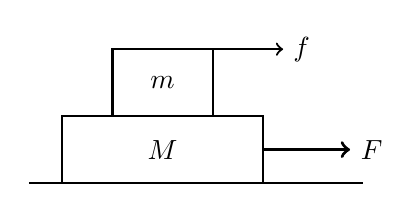
\begin{tikzpicture}[scale=.85]
\draw[thick] (-2,-1.8)--(3,-1.8);
\draw[thick] (-1.5,-1.8) rectangle (1.5,-.8);
\draw[thick] (-.75,-.8) rectangle (.75,.2);
\node at (0,-1.3) {$M$};\node at (0,-.3) {$m$};
\draw[->,very thick] (1.5,-1.3)--(2.8,-1.3) node[right] {$F$};
\draw[->,thick] (0,.2)--(1.8,.2) node[right] {$f$};
\end{tikzpicture}
\end{center}
\section{Ví dụ minh họa}
\subsection*{Ví dụ minh họa 1.1}
Hai vật: trên 2 kg, dưới 3 kg, sàn nhẵn. Lực ngang kéo vật dưới tăng dần. Lấy g=10 m/s\textsuperscript{2}, hệ số ma sát nghỉ 0,4 và trượt 0,3. Tìm ngưỡng và gia tốc hai vật khi lực 15 N và 30 N.

\textbf{Lời giải.} Không trượt cần $f=2F/5\le0{,}4(2)(10)=8$ N, suy ra $F_c=20$ N. Với 15 N, $a=15/5=3$ m/s\textsuperscript{2} và $f=6$ N, khả thi. Với 30 N cần ma sát nghỉ 12 N, không thể. Ma sát trượt 6 N hướng tới trước lên vật trên: $a_m=6/2=3$ m/s\textsuperscript{2}. Lên vật dưới hướng ngược: $a_M=(30-6)/3=8$ m/s\textsuperscript{2}. Vì $8>3$, chiều trượt nhất quán. Kiểm tra động lượng toàn hệ: $2(3)+3(8)=30$ N.
\subsection*{Ví dụ minh họa 1.2}
Vật 4 kg đang trượt trên sàn ngang. Lực 20 N kéo hợp góc θ phía trên ngang, hệ số ma sát trượt 0,25, g=10. Tìm góc cho gia tốc về trước lớn nhất và kiểm tra tiếp xúc.

\textbf{Lời giải.} Khi trượt về trước, $N=40-20\sin\theta>0$ với mọi góc cho phép. Gia tốc $a=[20(\cos\theta+0{,}25\sin\theta)-10]/4$. Viết $\cos\theta+0{,}25\sin\theta=\sqrt{1+0{,}25^2}\cos(\theta-\arctan0{,}25)$. Vậy $\theta=\arctan0{,}25\approx14{,}04^\circ$ và $a_{\max}=[20\sqrt{1{,}0625}-10]/4\approx2{,}654$ m/s\textsuperscript{2}. Tại cực đại $N\approx35{,}15$ N. Kết quả đúng khi vật còn trượt về trước.
\section{Luyện tập cuối chuyên đề}
\begin{enumerate}
\item \textbf{PHY202-A-1.1}. Vật trên 1 kg, dưới 4 kg; sàn nhẵn, hệ số nghỉ 0,5, trượt 0,3, g=10. Lực lên vật dưới lần lượt 20 N, 40 N. Tính gia tốc từng vật.
\item \textbf{PHY202-A-1.2}. Lập lại ngưỡng không trượt của hệ hai vật khi lực ngang F đặt lên vật trên m. Vật dưới M nằm trên sàn nhẵn.
\item \textbf{PHY202-A-1.3}. Thùng 5 kg trên mặt nghiêng 30\textdegree{}, hệ số nghỉ 0,4 và trượt 0,3. Ban đầu nghỉ, không có lực kéo. Xác định có trượt không và gia tốc nếu trượt. g=10.
\item \textbf{PHY202-A-1.4}. Vật đứng yên trên sàn xe tải ngang đang tăng tốc A. Suy ra hệ số ma sát nghỉ nhỏ nhất để vật không trượt. Giải thích trong cả hai hệ quy chiếu.
\end{enumerate}
\chapter{Liên kết, ròng rọc và chuyển động lăn}
\section{Lý thuyết và suy luận}
Với dây căng không dãn, viết phương trình hình học độ dài trước định luật Newton. Ròng rọc cố định hai nhánh thẳng đứng $y_1+y_2=L$ (cùng chọn xuống dương), đạo hàm hai lần cho $a_1+a_2=0$. Dây không khối lượng qua ròng rọc lý tưởng không khối lượng, không ma sát có lực căng bằng nhau; ròng rọc có khối lượng cần lực căng khác nhau để tạo moment. Điều kiện dây không trượt $a=R\alpha$. Các hệ thức này độc lập với định luật Newton và giúp khép kín hệ phương trình.

Với máy Atwood $m_2>m_1$, ròng rọc moment quán tính $I$, bán kính $R$, bỏ qua ma sát trục: $m_2g-T_2=m_2a$, $T_1-m_1g=m_1a$, $(T_2-T_1)R=I a/R$. Cộng cho $a=(m_2-m_1)g/(m_1+m_2+I/R^2)$. Tỉ số $I/R^2$ có thứ nguyên khối lượng, biểu thị quán tính quay, không phải trọng lượng. Khi $I\to0$, trở về ròng rọc lý tưởng; $I$ tăng thì $a$ giảm.

Vật rắn đối xứng trục khối lượng $m$, $I=\kappa mR^2$, lăn từ nghỉ xuống mặt nghiêng góc $\theta$. Chọn chiều tịnh tiến xuống dốc và chiều quay lăn dương: $mg\sin\theta-f=ma$, $fR=I a/R$ cho $a=g\sin\theta/(1+\kappa)$, $f=\kappa mg\sin\theta/(1+\kappa)$ hướng lên. Điều kiện $\mu_s\ge\kappa\tan\theta/(1+\kappa)$. Khi lăn thuần trên mặt cứng cố định, điểm tiếp xúc tức thời đứng yên nên ma sát nghỉ không sinh công trong hệ mặt đất. Phương trình năng lượng $mgh=(mv^2+I\omega^2)/2$ cho $v=\sqrt{2gh/(1+\kappa)}$. Chỉ dùng năng lượng không xác minh được ma sát nghỉ đủ hay không.

\section{Ví dụ minh họa}
\subsection*{Ví dụ minh họa 2.1}
Máy Atwood có hai vật 2 và 5 kg, ròng rọc là đĩa đồng chất 4 kg. Với g=10, tính gia tốc và hai lực căng.

\textbf{Lời giải.} Với đĩa $I/R^2=M_p/2=2$ kg. Quán tính hiệu dụng $2+5+2=9$ kg, lực phát động 30 N. Vậy $a=10/3$ m/s\textsuperscript{2}. $T_1=2(10+10/3)=80/3$ N, $T_2=5(10-10/3)=100/3$ N. Hiệu $20/3$ N bằng $(I/R^2)a=2(10/3)$, đúng điều kiện.
\subsection*{Ví dụ minh họa 2.2}
Trụ đặc đồng chất lăn từ nghỉ trên dốc 30\textdegree{} có độ cao 1,2 m. Lấy g=10. Tìm a, v ở chân dốc và hệ số ma sát nghỉ nhỏ nhất.

\textbf{Lời giải.} $\kappa=1/2$ cho $a=5/1{,}5=10/3$ m/s\textsuperscript{2}. Chiều dài dốc $1{,}2/\sin30^\circ=2{,}4$ m. Dùng $v^2=2as=16$, $v=4$ m/s. Năng lượng xác nhận $2gh/(1+\kappa)=16$. Cần $\mu_s=(1/3)\tan30^\circ=1/(3\sqrt3)\approx0{,}192$. Dưới giá trị này mô hình chỉ lăn không đúng.
\section{Nhiệm vụ thực nghiệm}
Dùng hai trụ bán kính gần nhau nhưng phân bố khối lượng khác nhau trên dốc thấp. Quay video từ nghỉ; đo quãng đường theo thời gian, fit s theo t\textsuperscript{2}, so sánh độ dốc với g sinθ/[2(1+κ)]. Đánh dấu vành, kiểm tra v≈Rω bằng video; nếu trượt, không diễn giải dữ liệu như lăn thuần. Báo cáo bất định góc, cản lăn, thời gian và độ lặp.
\section{Luyện tập cuối chuyên đề}
\begin{enumerate}
\item \textbf{PHY202-A-2.1}. Máy Atwood có hai vật 3 kg và 7 kg, ròng rọc đĩa 2 kg. Tìm a và các lực căng, g=10.
\item \textbf{PHY202-A-2.2}. Vành mỏng và cầu đặc, cùng khối lượng và bán kính, từ nghỉ lăn không trượt trên cùng dốc. Suy ra tỉ số gia tốc và tỉ số tốc độ ở chân dốc.
\item \textbf{PHY202-A-2.3}. Trụ đặc thả trên dốc có tan θ=0,6, hệ số nghỉ 0,15 và trượt 0,10. Xác định lăn thuần có khả thi không. Nếu không, tìm gia tốc tịnh tiến và góc ban đầu theo g và R.
\item \textbf{PHY202-A-2.4}. Ròng rọc động nhẹ đỡ tải 6 kg bằng hai nhánh dây thẳng đứng. Đầu tự do được kéo xuống 0,8 m với tốc độ không đổi trong hệ lý tưởng. Tìm độ nâng tải, lực căng và công đầu vào; g=10.
\end{enumerate}
\chapter*{Tài liệu và bài đọc mở rộng}\addcontentsline{toc}{chapter}{Tài liệu và bài đọc mở rộng}
VPhO 2001 nhóm 1 bài 1.1 (trang in 5); VPhO 2003 nhóm 5 bài 5.1 (tr. 14–15); VPhO 2008 nhóm 14 bài 14.1 (tr. 36); VN TST 2003 nhóm 21 bài 21.1 (tr. 56–58). Đây là chỉ mục đến tuyển tập đính kèm, không phải nguồn của bài tự biên soạn trong tập.

\url{https://diavn.github.io/truongchuyen/physics-vpho.html}

\url{https://hyperphysics.gsu.edu/hbase/hph.html}

\url{https://openstax.org/subjects/science}
\appendix
\chapter{Lời giải đầy đủ phần luyện tập}
\section{Định luật Newton và các chế độ ma sát}
\begin{enumerate}
\item \textbf{PHY202-A-1.1}. Ngưỡng $F_c=0{,}5(5)10=25$ N. Với 20 N, cả hai gia tốc 4 m/s\textsuperscript{2}, cần ma sát 4 N. Với 40 N, $f_k=3$ N, $a_m=3$ m/s\textsuperscript{2}, $a_M=(40-3)/4=9{,}25$ m/s\textsuperscript{2}. Vật dưới đi trước; kiểm tra $1(3)+4(9{,}25)=40$ N.
\item \textbf{PHY202-A-1.2}. Không trượt vẫn cho $a=F/(M+m)$. Ma sát lên vật dưới phải cung cấp $Ma=MF/(M+m)$. Vì $N=mg$, điều kiện $MF/(M+m)\le\mu_smg$, tức $F_c=\mu_smg(M+m)/M$. Vượt ngưỡng $a_M=\mu_kmg/M$, $a_m=(F-\mu_kmg)/m$. Công thức khác trường hợp kéo dưới vì vật được truyền lực qua ma sát khác.
\item \textbf{PHY202-A-1.3}. $N=mg\cos30^\circ=25\sqrt3$ N; thành phần trọng lực xuống dốc $mg\sin30^\circ=25$ N. Ma sát nghỉ cực đại $10\sqrt3\approx17{,}32$ N không đủ. Ma sát trượt $7{,}5\sqrt3$ N lên dốc. Vậy $a=(25-7{,}5\sqrt3)/5=5-1{,}5\sqrt3\approx2{,}40$ m/s\textsuperscript{2} xuống dốc.
\item \textbf{PHY202-A-1.4}. Hệ mặt đất: ma sát về trước cần $f=mA$, $N=mg$, nên $\mu_s\ge A/g$. Hệ xe: vật đứng yên, lực quán tính $-mA$ cân bằng $f=mA$. Cả hai cho cùng điều kiện tiếp xúc. Dấu bằng là giới hạn sắp trượt.
\end{enumerate}
\section{Liên kết, ròng rọc và chuyển động lăn}
\begin{enumerate}
\item \textbf{PHY202-A-2.1}. $I/R^2=1$ kg; $a=40/11$ m/s\textsuperscript{2}. $T_1=3(10+40/11)=450/11$ N, $T_2=7(10-40/11)=490/11$ N. Hiệu $40/11$ N tạo moment cho ròng rọc.
\item \textbf{PHY202-A-2.2}. $\kappa_h=1$, $\kappa_s=2/5$. Vậy $a_s/a_h=(1+1)/(1+2/5)=10/7$. Cùng độ giảm độ cao, $v_s/v_h=\sqrt{10/7}$. Hai kết quả yêu cầu ma sát nghỉ đủ đối với từng vật.
\item \textbf{PHY202-A-2.3}. Lăn thuần cần $\mu_s\ge\tan\theta/3=0{,}2$, nên không khả thi. Trọng lực gây trượt điểm tiếp xúc xuống dốc, ma sát hướng lên. $\cos\theta=1/\sqrt{1{,}36}$, $\sin\theta=0{,}6/\sqrt{1{,}36}$. Do đó $a=g(\sin\theta-0{,}1\cos\theta)=0{,}5g/\sqrt{1{,}36}$; $\alpha=fR/I=0{,}2g/(R\sqrt{1{,}36})$. Vì $a-R\alpha=0{,}3g/\sqrt{1{,}36}>0$, chiều trượt giả định đúng.
\item \textbf{PHY202-A-2.4}. Liên kết độ dài dây $2y+x=\text{hằng số}$ với tọa độ tải $y$ và đầu dây $x$ cùng chiều dương xuống. Vậy $\Delta y=-0{,}4$ m: tải nâng 0,4 m. Tốc độ không đổi cho $2T=mg=60$ N, nên $T=30$ N. Công đầu vào $T(0{,}8)=24$ J, bằng $mgh=6(10)(0{,}4)=24$ J.
\end{enumerate}
\end{document}
